\chapter{Characteristics of OpenStreetMap}
Important information when looking at how to import external data into OpenStreetMap is understanding the data structure of OpenStreetMap. This data structure is unique and only supported by OSM. This chapter will give an introduction to this structure. It will also cover how this data structure is realized through the XML format. When importing data into OSM the original data needs to be converted into XML files supporting this data structure. Since this study will look at FKB building data it is important to understand how to map buildings in OpenStreetMap, both in 2D and 3D. This will also be covered in this chapter. 

\section{Data structure}\label{sec:datastructure}
OpenStreetMap uses a topological data structure. This structure includes three basic components nodes, ways, and relations. Nodes are points with a geographic position stored as coordinates (Lat, long) according to WGS84. Ways are lists of two or more nodes, representing an open- or closed way used to describe streets, rivers, among others \cite{Debruyne2015}. A relation is a multi-purpose data structure that documents a relation between two or more components \cite{OpenStreetMapg}. OpenStreetMap's structure uses tags to add metadata to geographic objects. Tags consist of two items, a key and a value of the form key=value. The key is used to describe the topic, category or type of feature, while the value represents the details of the particular form of the key specified. An example of a key-value pair can be building=church, here the key is building and the value is a church, this is a building that was built as a church. 

OpenStreetMap does not have any restrictions on tags assigned to nodes, ways or relations, and mappers can use any key-value pair in their import. Nevertheless, the norm in OSM is to try to map new data with existing tags. Good practice is to search for tags, or map features, on different OSM wiki pages. On the \textit{tags you like} wiki page they recommend different pages, but points out \textit{taginfo.openstreetmap.org} as the most useful site. Taginfo is a website created for finding and aggregating information about OSM tags, it covers the whole planet and is updated daily. The web page list tags used in the database and also information on how frequent they appear in the OSM database. Taginfo also lists other tags which have been used in combination with the displayed tag. Some countries also have their own taginfo web pages, like Ireland, Great-Britain, and France, Norway does not have it. If a mapper doesn't find an appropriate key-value pair and wants to create a new feature, this has to be documented on the OSM wiki page. 

In OSM, changes made by one user over a short period is called a changeset \cite{OpenStreetMapi}. A change can be a creation of new components, adding tags to existing components, changes to tags in existing components, removal of tags and removal of components. Changes are added to the changeset as long as it's open, changesets are either closed directly or by itself after a period of inactivity (currently after one hour). Every component edit in the OSM database is a part of a changeset.

 \section{File format, .osm files}\label{sec:osmxml}
The .osm file format is specific to OpenStreetMap, and it is not easy to open these files using GIS-software like QGIS. The file format is designed to be easily sent and received across the Internet in a standard format. Therefore .osm files are easily obtained, but using the files directly for analyzing and map design is not easy. The .osm files are coded in the XML format. It is recommended to convert the data into other formats when using the files \cite{Learnosm}. 

Nodes, ways and relations is represented by their own tag: <node>, <way> and <relation>. When nodes are used on their own, which means that they are not included in a way or a relation, they represent point features. Points features normally include at least one tag to define the points purpose \cite{OpenStreetMapc}. In listing \ref{eq:nodetag} the node tag describes a bag shop named Citybag, this is called a point of interest. The key named user give the name of who last modified this node (user="Peter Bremer") and uid is the person's numeric user id (uid="366321").


\lstset{
    language=XML,
    morekeywords={encoding,node, tag},
    label=eq:nodetag,
    caption=Example of a node tag
}
\begin{lstlisting}
 <node id="4004323486" visible="true" version="1" changeset="37189343"
  timestamp="2016-02-13T15:58:54Z" user="Peter Bremer" uid="366321" 
  lat="63.4318129" lon="10.3971411">
  <tag k="name" v="Citybag"/>
  <tag k="shop" v="bag"/>
 </node>
\end{lstlisting}

A way-tag consists of two or more nodes and can either be open or closed. An open way describes a line feature that does not share the first and last node. When a way is closed the first and last nodes are the same and can be interpreted as a closed polyline or an area, or both \cite{OpenStreetMapd}. A closed way with highway=* tag can represent roundabouts, or if it has amenity=school tag the closed way represent the outline of a school. In listing \ref{eq:waytag1} the way describes the building outline of a church since the key equals building and the value equals church. The <nd> tag represents a node, where the <nd> tags refers to <node> tags who contains the lat, long values. All <nd> tags create the building footprint, notice that there is no height parameter. Listing \ref{eq:waytag1} creates a 2D representation of the church which is shown in figure \ref{fig:fruekirke2D}. A 3D representation of the same church is shown in figure \ref{fig:fruekirke}.

\lstset{
    language=XML,
    morekeywords={encoding, relation, way, tag, node, member},
    label=eq:waytag1,
    caption=Example of a way tag - creating the building footprint of a church
}
\begin{lstlisting}
 <way id="89340594" visible="true" version="6" changeset="42571811" 
  timestamp="2016-10-01T22:11:17Z" user="Peter Bremer" uid="366321">
  <nd ref="1036369169"/>
  <nd ref="1036369134"/>
  <nd ref="1036369111"/>
  <nd ref="1036369185"/>
  <nd ref="1036369163"/>
  <nd ref="1036369118"/>
  <nd ref="1036369099"/>
  <nd ref="4427055078"/>
  <nd ref="1036369179"/>
  <nd ref="1036369158"/>
  <nd ref="4427055082"/>
  <nd ref="1036369145"/>
  <nd ref="1036369124"/>
  <nd ref="1036369103"/>
  <nd ref="4215548739"/>
  <nd ref="4215548736"/>
  <nd ref="4215548737"/>
  <nd ref="4215548740"/>
  <nd ref="1036369182"/>
  <nd ref="1036369140"/>
  <nd ref="1036369115"/>
  <nd ref="1036369096"/>
  <nd ref="1036369135"/>
  <nd ref="1036369149"/>
  <nd ref="4427055803"/>
  <nd ref="1036369131"/>
  <nd ref="1036369107"/>
  <nd ref="1036369169"/>
  <tag k="amenity" v="place_of_worship"/>
  <tag k="building" v="church"/>
  <tag k="denomination" v="protestant"/>
  <tag k="name" v="Vår Frue kirke"/>
  <tag k="religion" v="christian"/>
  <tag k="wheelchair" v="yes"/>
  <tag k="wikidata" v="Q3356455"/>
  <tag k="wikipedia" v="en:Vår Frue Church"/>
 </way>
\end{lstlisting}

\begin{figure}[H]
    \centering
    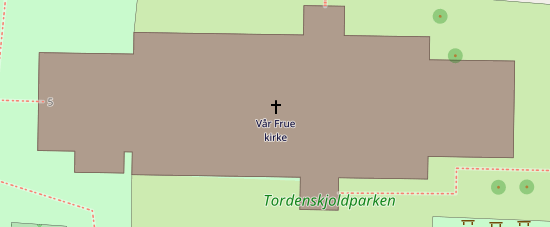
\includegraphics[scale=0.5]{figures/FixedByMe/fruekirke2D.png}
    \caption{2D representation of \textit{Vaar frues kirke}, result of listing \ref{eq:waytag1}. Source: \cite{OpenStreetMap2016b}}
    \label{fig:fruekirke2D}
\end{figure}

A relation is an ordered list of one or more nodes, ways, and/or relations and is used to define logical or geographical relationships between the other elements \cite{OpenStreetMape}. If a building consists of multiple parts, tagged with building:part=*, a relation is used to define the geographical relationship between the parts. Specifying roles to different parts is possible. A road can have the role as east, going towards the east. In multi-polygons, parts can have an inner or outer role, to specify whether it forms the inner or outer part of the polygon. A building relation is shown in listing \ref{eq:reltag}. There are eight members in this relation. The first member is a way, and it has an outline role creating the building footprint, used as 2D representation of the church. Listing \ref{eq:waytag1} is the XML-code for this outline (notice that the ref number \textit{89340594} are equal to the way id in listing \ref{eq:waytag1}). The only node member in the relation contains the church's address. The rest of the members creates the 3D representation of the church shown in figure \ref{fig:fruekirke}.

\lstset{
    language=XML,
    morekeywords={encoding, relation, way, tag, node, member},
    label=eq:reltag,
    caption=Example of a relation tag - creating 3D representation of a church
}
\begin{lstlisting}
 <relation id="6269954" visible="true" version="2" changeset="39708156" 
  timestamp="2016-06-01T11:14:18Z" user="Peter Bremer" uid="366321">
  <member type="way" ref="89340594" role="outline"/>
  <member type="node" ref="2957446972" role=""/>
  <member type="way" ref="421821942" role=""/>
  <member type="way" ref="421821938" role=""/>
  <member type="way" ref="421821939" role=""/>
  <member type="way" ref="421821940" role=""/>
  <member type="way" ref="421821937" role=""/>
  <member type="way" ref="421821941" role=""/>
  <tag k="name" v="Vår Frue kirke"/>
  <tag k="type" v="building"/>
 </relation>
\end{lstlisting}

\begin{figure}[H]
    \centering
    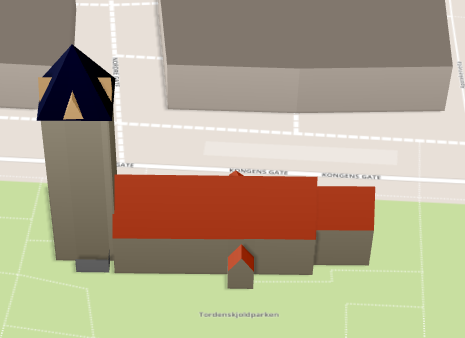
\includegraphics[scale=0.5]{figures/FixedByMe/fruekirke.png}
    \caption{3D representation of \textit{Vaar frues kirke}, result of listing \ref{eq:reltag}. Source: \cite{Buildings2016}}
    \label{fig:fruekirke}
\end{figure}


 \section{Mapping buildings in OSM}\label{buildOSM}
A building can be represented by nodes, ways or relations in OpenStreetMap. When importing buildings into OSM, the XML-code representing the building must be tagged with Building=*. Frequent occurring values are house, residential and garage, describing the buildings particular usage.  Using the building tag in node representations is tolerated but not recommended. A building is much better expressed by their footprint (close way or multi-polygon), and if the footprint is available, one should not add the building key in nodes. The building key should be used to mark the footprint of the building. The most common occurring value for the building key is yes and used when it's not possible to determine a more accurate value \cite{OpenStreetMapf}. A list of possible values that can be added to the building key is listed on the OSM \textit{building} wiki page. It is possible to introduce new values, but it is not recommended. The building key is most common used in way representations \cite{TagInfo2016}. An example of how to use building key in a way tag see listing \ref{eq:waytag1}.

Relations is used if the building consists of multiple parts which physical differ from each other, often when a 3D representation of the building is created. A building relation mainly consists of two or more ways. A way then represents a part of the building and should be tagged with a building:part key and usually the value yes. Then the way-tags representing the different building parts are ordered together inside the relation. An example of a building:part=yes implementation can be seen in listing \ref{eq:waytag}. Note that the first and last <nd> tag refers to the same node, so this is a closed way. The key roof:shape with value gable gives the appearance of the roof. The result from the code in listing \ref{eq:waytag} is shown in figure \ref{fig:erkeinng} marked with a red line. A relation containing building:parts are shown in listing \ref{eq:reltag}. Notice that this relation is tagged with the key type and the value building. If a relation is tagged with type=building, it groups both building footprint and all building parts together. See figure \ref{fig:fruekirke} for a 3D building representation created with building parts. 

\lstset{
    language=XML,
    morekeywords={encoding,way, tag, nd},
    label=eq:waytag,
    caption=Example of a way tag - creating 3D representation of a building part
}
\begin{lstlisting}
  <way id="17533469" visible="true" version="22" changeset="39301425" 
  timestamp="2016-05-13T21:20:04Z" user="Peter Bremer" uid="366321">
  <nd ref="3505716655"/>
  <nd ref="2517225923"/>
  <nd ref="4184346715"/>
  <nd ref="3505716656"/>
  <nd ref="4184346713"/>
  <nd ref="4184346717"/>
  <nd ref="3505716654"/>
  <nd ref="4184346719"/>
  <nd ref="3505716655"/>
  <tag k="building:colour" v="#c3c0b9"/>
  <tag k="building:material" v="stone"/>
  <tag k="building:part" v="yes"/>
  <tag k="height" v="11"/>
  <tag k="name" v="Sydkapell"/>
  <tag k="roof:height" v="4"/>
  <tag k="roof:material" v="copper"/>
  <tag k="roof:orientation" v="across"/>
  <tag k="roof:shape" v="gabled"/>
 </way>
\end{lstlisting}

\begin{figure}[H]
    \centering
    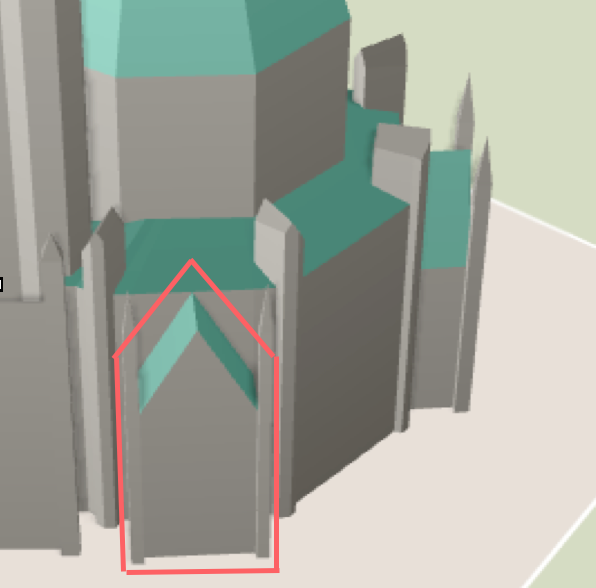
\includegraphics[scale=0.5]{figures/FixedByMe/nidaros3D.png}
    \caption{\textit{Sydkapell} with gabled shaped roof, result of listing \ref{eq:waytag}. Source: \cite{Buildings2016}}
    \label{fig:erkeinng}
\end{figure} 